\documentclass{article}

\usepackage{url}
\usepackage{tikz}
\usepackage{float}
\usepackage{amsmath}
\usepackage{enumitem}

\usetikzlibrary{matrix, shapes, snakes, arrows}
\tikzset{>=triangle 45}

\title{CS 612: Assignment 2\\Spring 2013}

\author{Dustin Ingram}

\date{\today}

\begin{document}

\maketitle

\section*{Written}

\begin{enumerate}

\item{} % 1

I would equip the robots with simple sensors to detect radioactivity at a
specific location (such as a digital Geiger counter). I will assume that the
robots have no other means of control or inter-communication. The large number
of robots will go into the plant with a small number of pellets, drop them at
some location, and return for more pellets. When the robots enter the plant for
the first time, they will travel randomly within it. This is for two reasons:
one, because it is initially unknown where the highly radioactive areas are, and
two, because it is unknown how radioactive the most radioactive areas are. The
robots travels randomly for a set period of time to determine an average
radioactivity for the area. It then proceeds to continue moving randomly until
it finds an area which is more radioactive than the average it has found. When
it has found such a location, it will drop the pellets, thus reducing the
overall average radioactivity for the area it has seen, and leave for more
pellets. The entire time the robot is moving, it will be continually updating
it's running average, to have a better knowledge of the true radioactivity of
the space. As each robot places their pellets, the total actual average
radioactivity of the plant will decrease. Once the robots find no place within
the plant whose maximum radioactivity exceeds the allowable radioactivity within
a given amount of time, it will leave and the plant will be considered safe.

\item{} % 2

The key concepts from actual ant behavior that are used in most ant colony
optimization algorithms are:

\begin{itemize}
    \item Random initial search - Without any initial pheromone trails, scout
    ants will randomly (or quasi-randomly) move about their environment in
    search of food. This ensures eventually finding a food source and returning
    to the nest;
    \item Pheroemone laying - Actual ants, once they have found a food source,
    will leave a trail of pheromones from the food to the nest. This serves as a
    path for other ants to follow, to strengthen the path to the food;
    \item Collective pheromones - In actual ant systems, ants to not have unique
    pheremones, so multiple ants laying pheromones in the same location will
    simply multiply the ``signal'' for that location, allowing a good path to be
    strengthened;
    \item Pheromone decay - In the real world, pheromones decay and dissipate
    over time. While this may degrade a path to a good solution, it also ensures
    that longer or less frequently traveled paths to the same location are less
    desirable for any given ant than a more optimal path.
    \item Path following - Actual ants have the ability to detect a pheromone
    trail, and to follow it from it's source to it's destination. This allows
    ants to intelligently follow a path laid by their predecessors.
    \item Deviations - Actual ants aren't perfect at following the trail,
    though, and may deviate from it. This helps ants find a possibly shorter
    path than the one they should be following.
\end{itemize}

\item{} % 3

To adapt a particle swarm optimization problem to a dynamic or ``online''
solution, my main focus would be to allow the system to determine when there has
been a change in the system, and tell the particles to discard or re-determine
their best positions and velocities accordingly. By being able to discard this
outdated memory of the optimal solution, the particles will be able to
re-optimize to find a new solution every time the problem changes.

\end{enumerate}

\section*{Programming}

For my solution, I used the Ant Colony Optimization algorithm, exactly as it
was given in the slides.

The control parameters for my implementation are as follows:

\begin{align*}
    \alpha &= 1.0\\
    \beta &= 10.0\\
    \rho &= 0.1\\
    Q &= 1.0\\
    n_{ants} &= 5
\end{align*}

I arrived at these parameters after trying a few values and seeing which ones
solved the Djibouti case the fastest. If I had more time, I would likely specify
a range and a step for each of these, and attempt to see which combination of
each (out of possibly hundreds) actually performed the best.

\begin{enumerate}

\item{} % 1

For the Djibouti case, my implementation is able to converge, on average, within
0.2\% of the optimal solution. The best run of my implementation was able to
converge on the optimal solution. To generate this statistic, I ran my
implementation 30 times, giving it 5 seconds to complete.

\item{} % 2

For the Luxembourg case, my implementation is able to converge, on average,
within 28\% of the optimal solution. The best run of my implementation was
a length of 14353. To generate this statistic, I ran my implementation 10 times,
giving it 120 seconds to complete.

\item{} % 3
For the Argentina case, my implementation is able to converge, on average,
within 29\% of the optimal solution. The best run of my implementation was
a length of 1087557. To generate this statistic, I ran my implementation one
time, giving it over two hours to complete.

\item{} % 4
The accuracy for Argentina definitely improves over time, but the simulation
takes a very long time. The following graph does not have confidence intervals
because I only had time to run a single simulation (it took approx. 2 hours).

\begin{figure}[H]
\centering
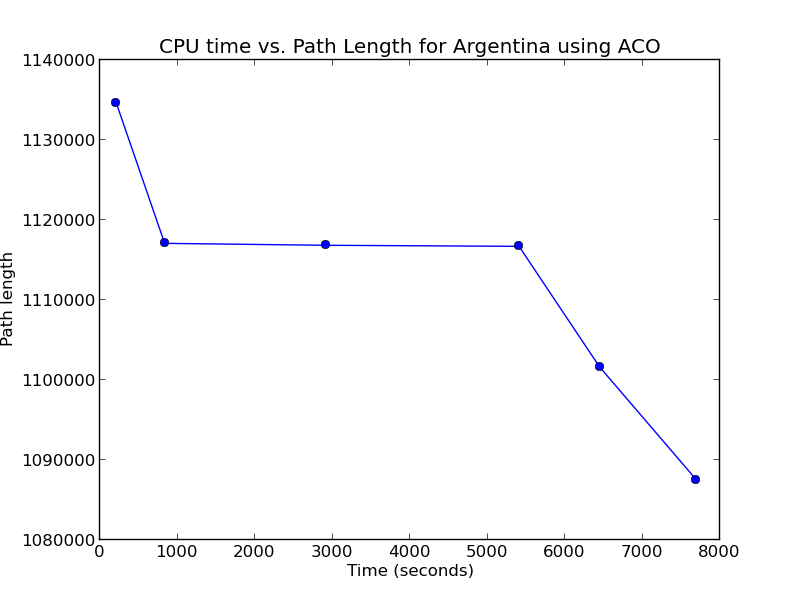
\includegraphics[width=\textwidth]{figs/figure_1.png}
\caption{Five ants touring 9152 cities after 2 hours. }
\end{figure}

\end{enumerate}

\end{document}
